\documentclass[final,nototal,pdf,mark]{prosper}
\title{Object Oriented NeXus Classes }
\author{Mark K\"onnecke}
\institution{Laboratory for Development and Methods\\Paul Scherrer Institut}
\Logo{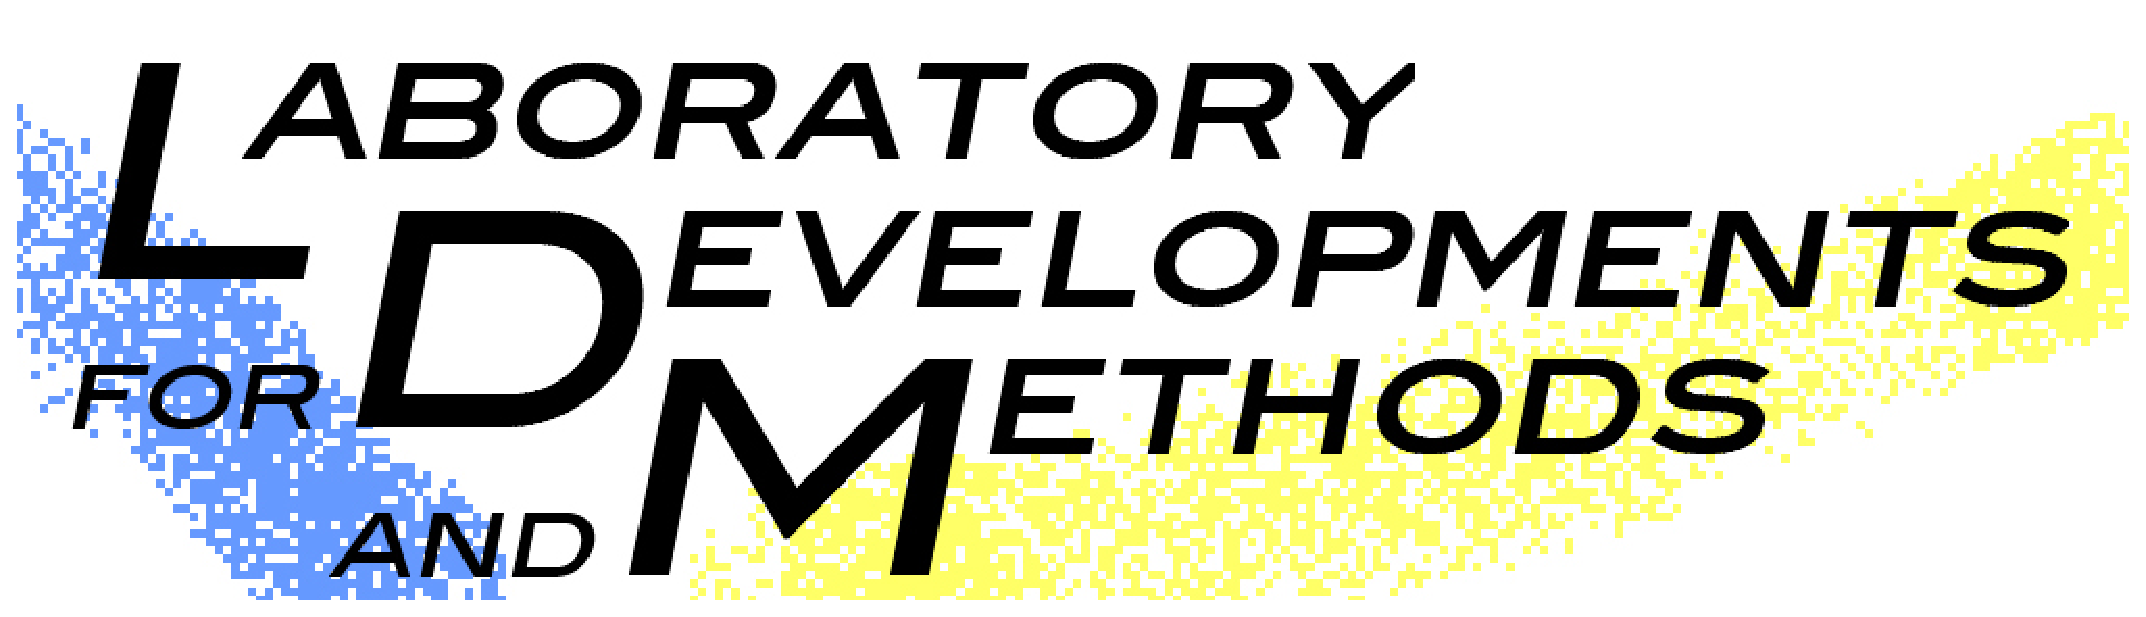
\includegraphics[width=4cm]{ldmlogo.eps}}

\begin{document}
\maketitle



\begin{slide}{Simple Coordinate System }
\begin{itemize}\item The plane perpendicular to the main rotation axis of the sample table def\mbox{}ines the 
 scattering plane of the instrument.  
\item As components are commonly positioned using angles, a polar coordinate system is used.
\item When distances are required then we assume that the sample is a zero. Distances towards the
 source are negative, distances behind the sample, towards the detector are positive.  
\end{itemize}
\end{slide}\begin{slide}{Polar Angle, Distance and Rotation }
\begin{itemize}\item The angle between the extension of the direct beam between a given component and its previous 
 component  and the projection of a third component onto the scattering plane is the polar\_angle. This 
 corresponds to longitude in a a geographical coordinate system. In scattering this is synonymous with 
 two theta or gamma in normal beam geometry.
\item Birds eye view on scattering plane:
\end{itemize}\begin{center}
\begin{figure}
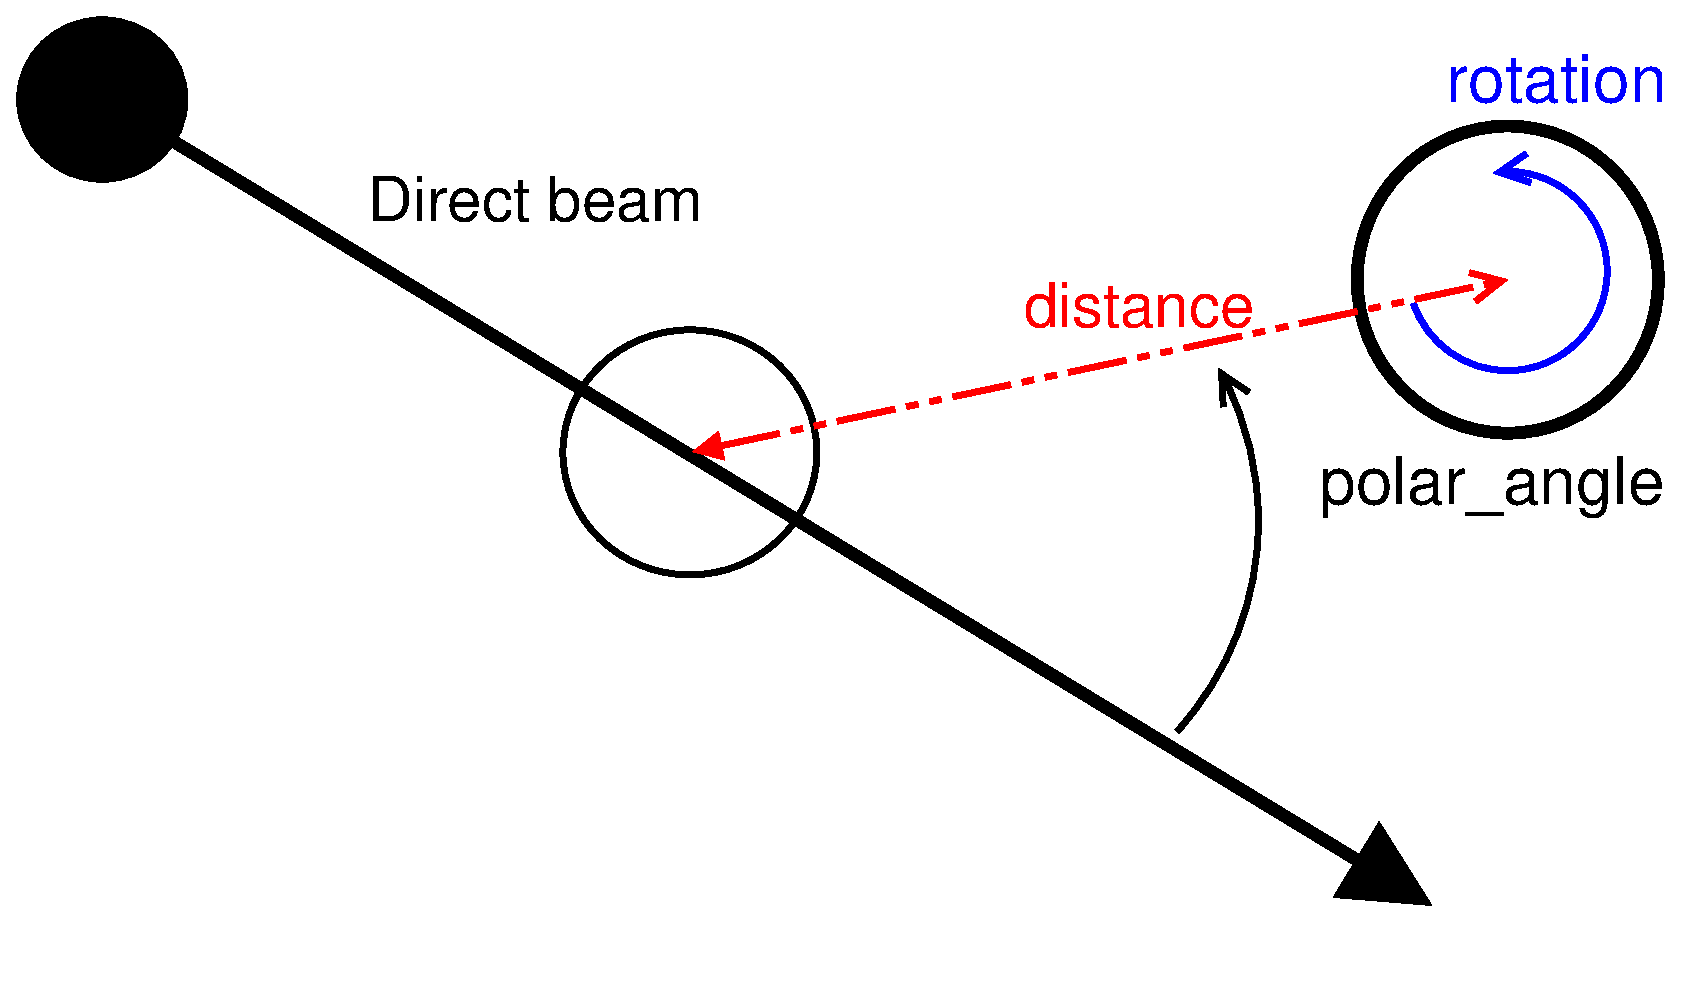
\includegraphics[width=0.75\textwidth]{polar.eps}\end{figure}



\end{center}

\end{slide}\begin{slide}{Elevation }
\begin{itemize}\item Standing besides the instrument:
\end{itemize}\begin{center}
\begin{figure}
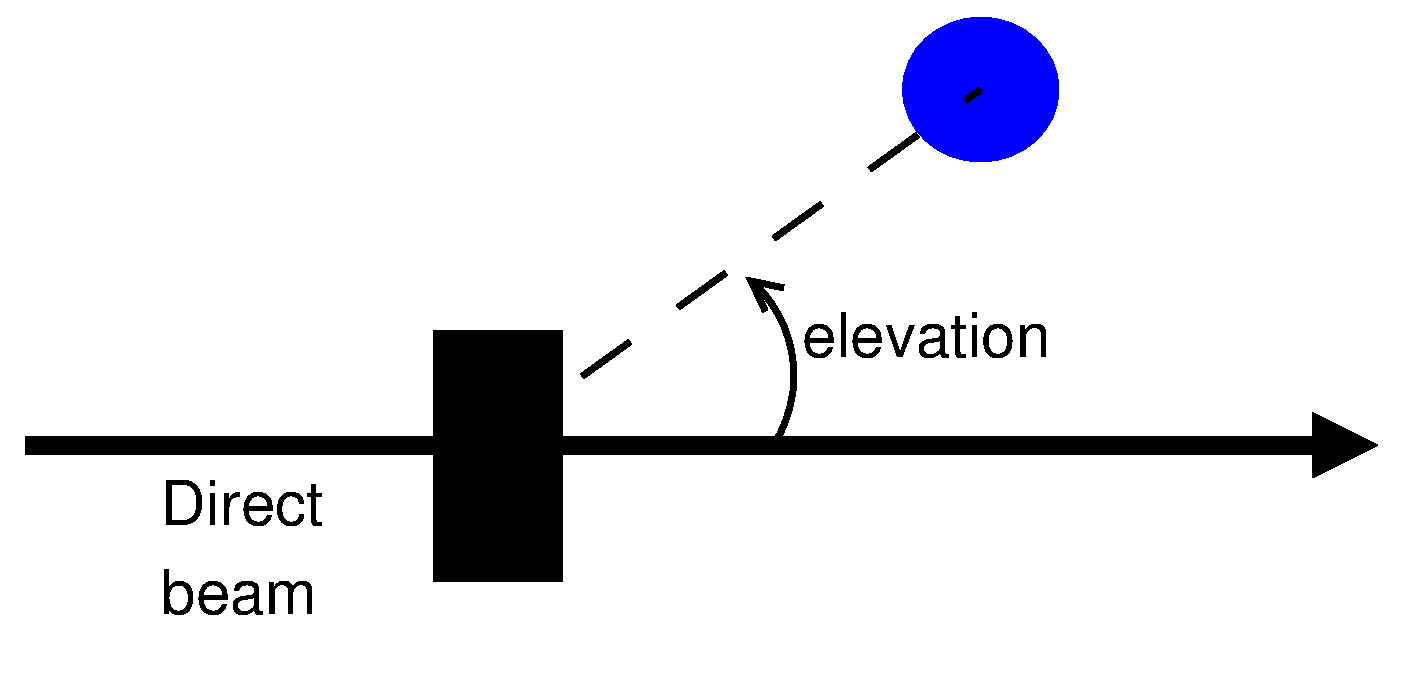
\includegraphics[width=0.75\textwidth]{elevation.eps}\end{figure}



\end{center}
\begin{itemize}\item Elevation corresponds to latitude in geography. In neutron scattering this is often the angle nu.
\end{itemize}
\end{slide}\begin{slide}{Azimuthal Angle }
\begin{itemize}\item Again birds eye view onto the scattering plane
\end{itemize}\begin{center}
\begin{figure}
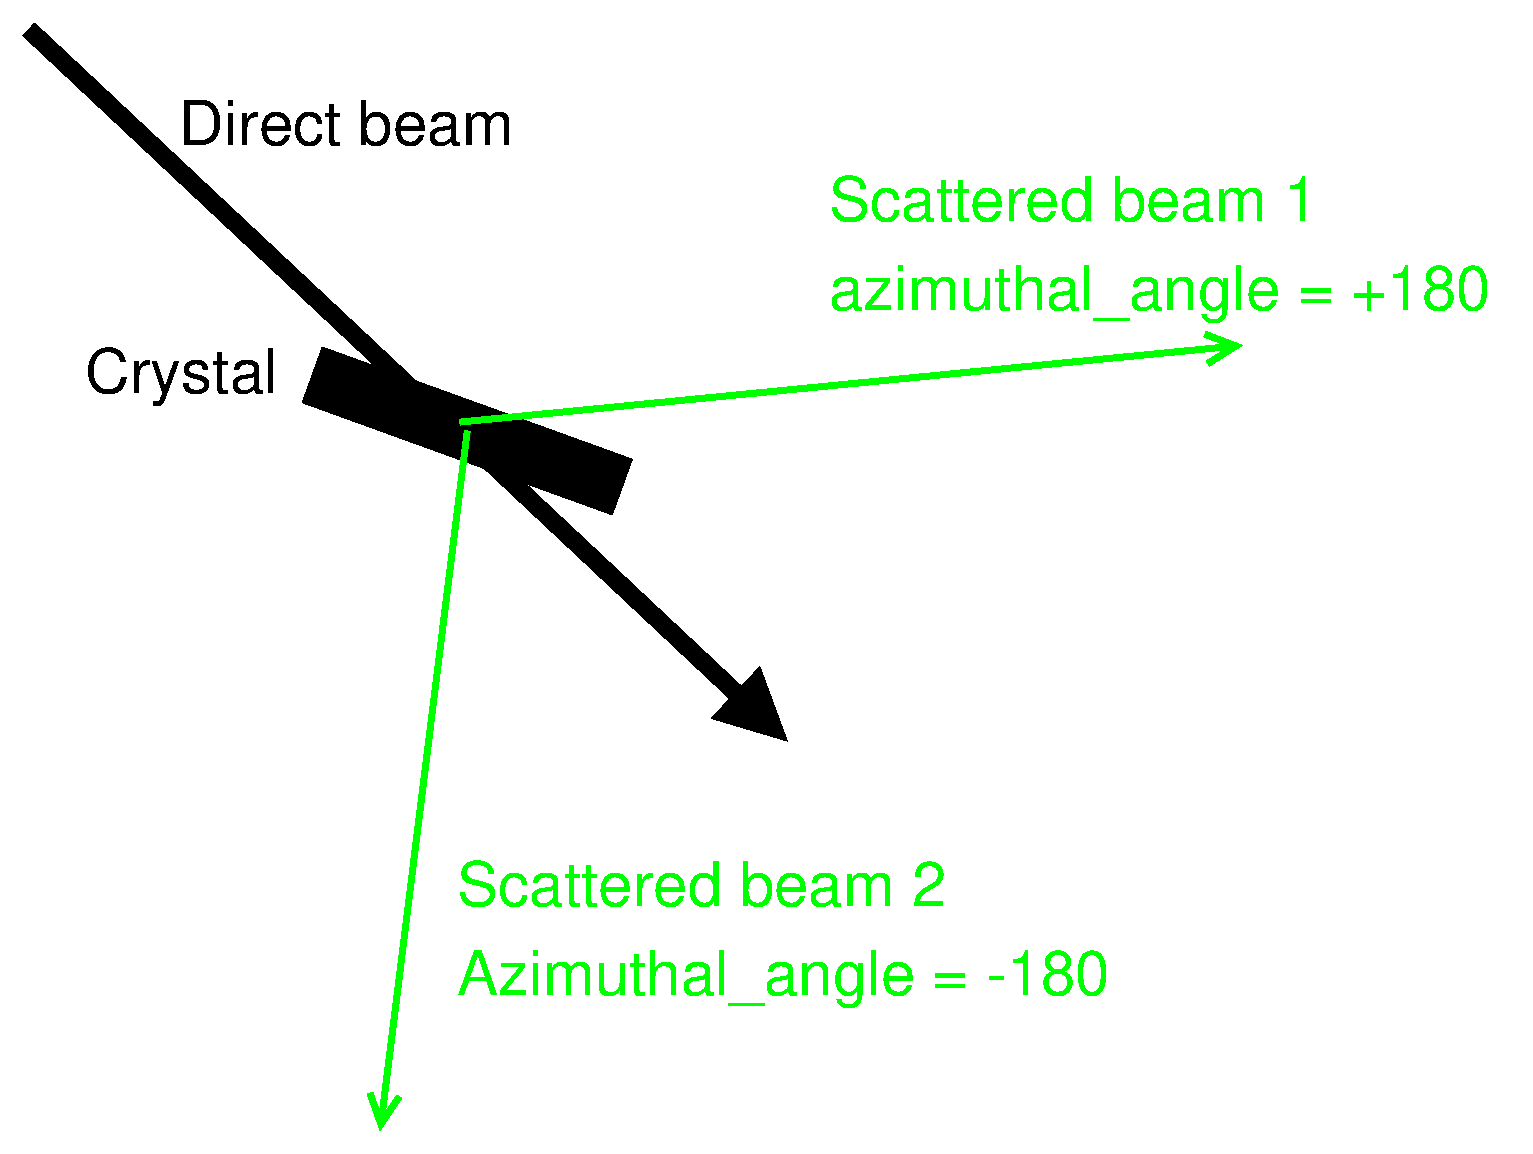
\includegraphics[width=0.75\textwidth]{azimuthal.eps}\end{figure}



\end{center}

\end{slide}\begin{slide}{McStas Coordinates }
\begin{itemize}\item Birds eye view again:
\end{itemize}\begin{center}
\begin{figure}
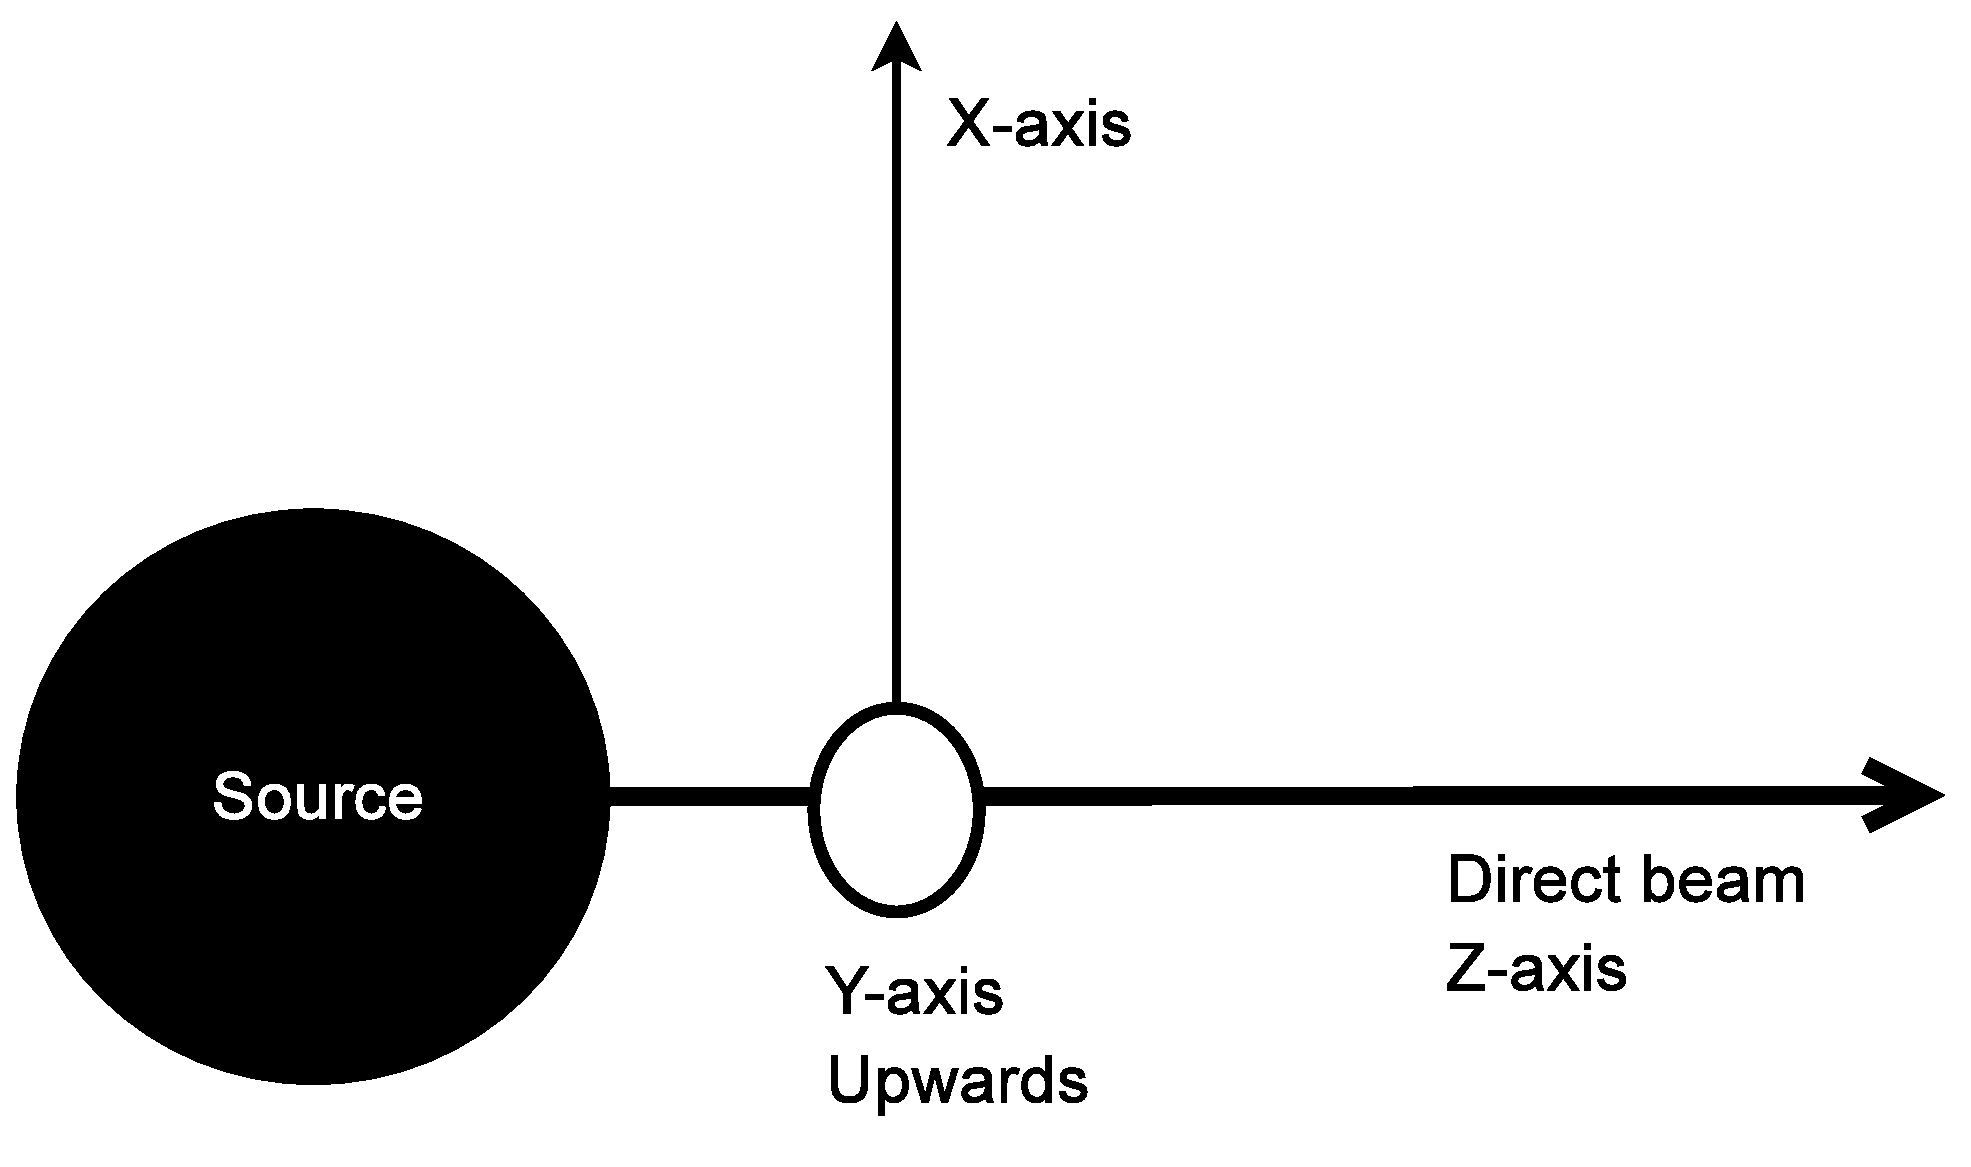
\includegraphics[width=0.75\textwidth]{mcstas.eps}\end{figure}



\end{center}
\end{slide}\begin{slide}{Miscellaneous Classes }
\begin{center}
\begin{figure}
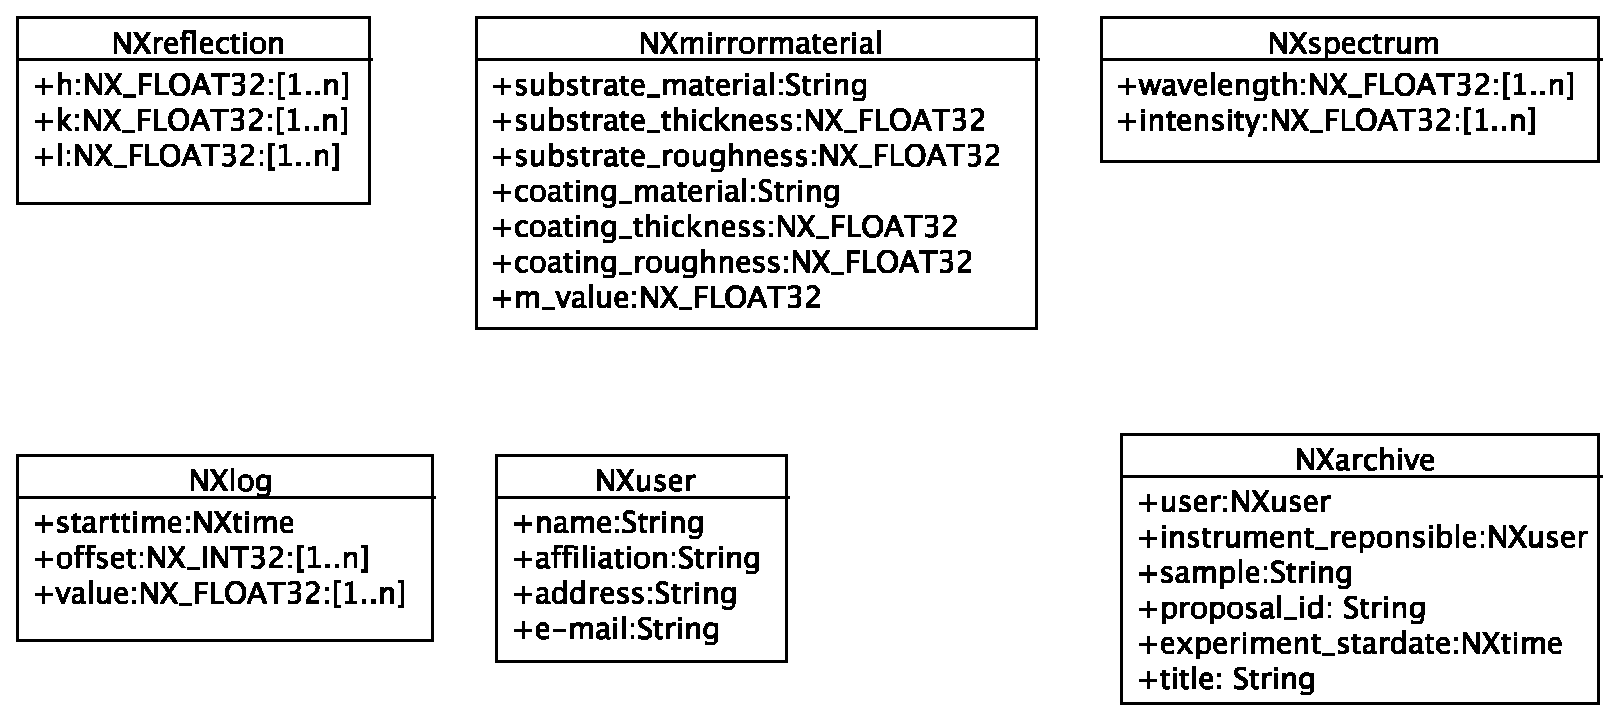
\includegraphics[width=0.75\textwidth]{nxmisc.eps}\end{figure}



\end{center}
\end{slide}\begin{slide}{NeXus Position }
\begin{center}
\begin{figure}
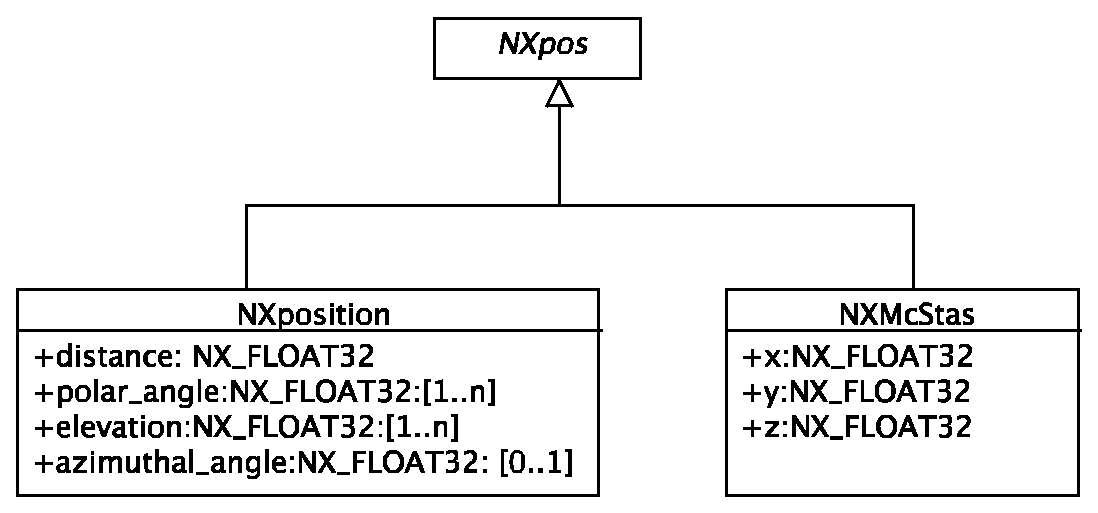
\includegraphics[width=0.75\textwidth]{nxpos.eps}\end{figure}



\end{center}

\end{slide}\begin{slide}{NeXus Shape }
\begin{center}
\begin{figure}
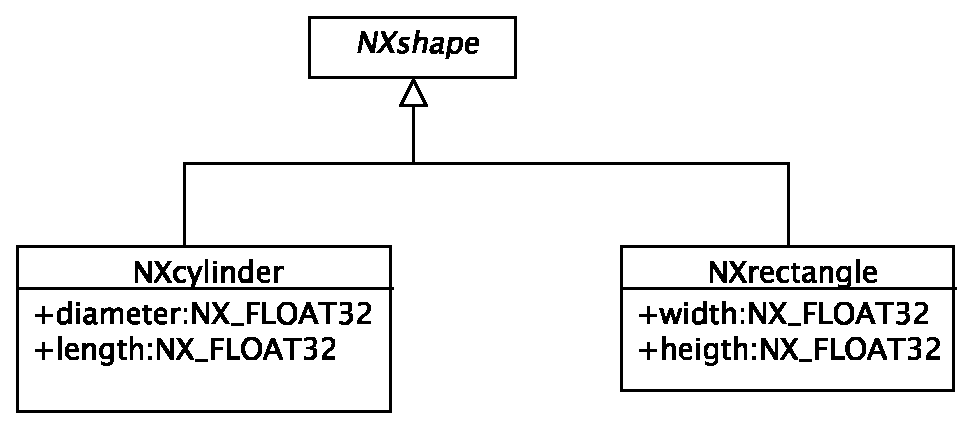
\includegraphics[width=0.75\textwidth]{nxshape.eps}\end{figure}



\end{center}
\end{slide}\begin{slide}{NeXus Stages }
\begin{center}
\begin{figure}
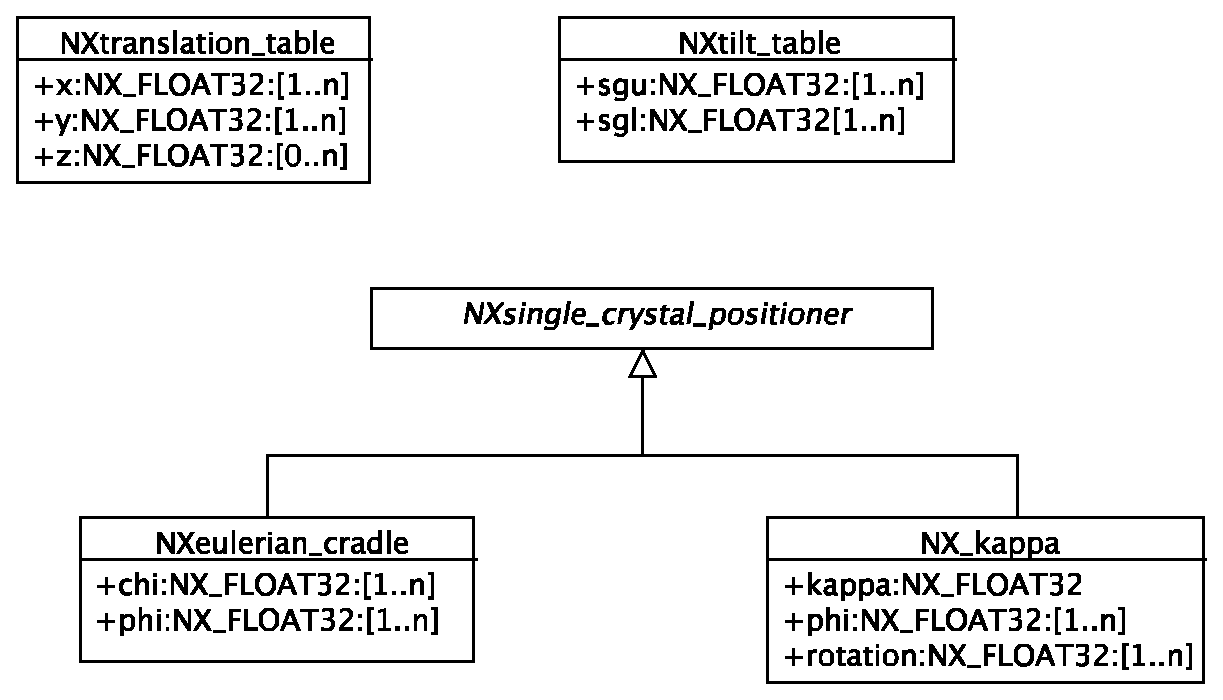
\includegraphics[width=0.75\textwidth]{nxstage.eps}\end{figure}



\end{center}
\end{slide}\begin{slide}{Source Components }
\begin{center}
\begin{figure}
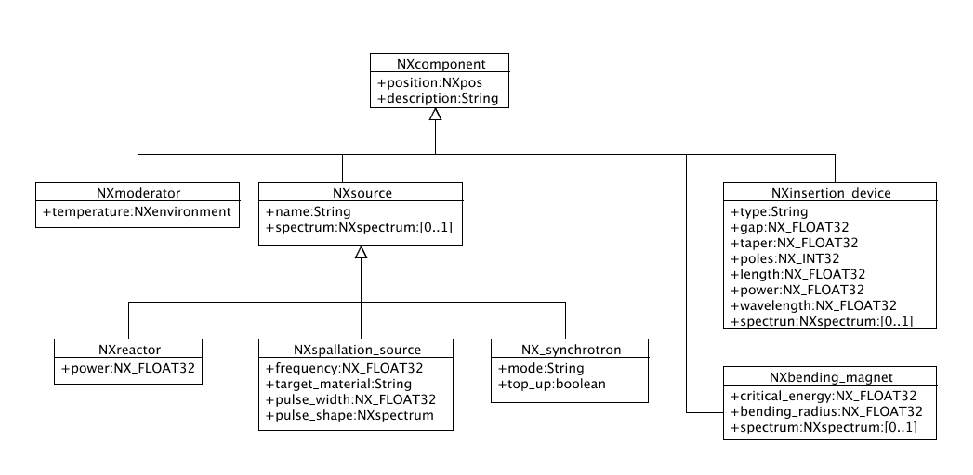
\includegraphics[width=0.75\textwidth,height=0.75\textheight]{nxsource.eps}\end{figure}



\end{center}

\end{slide}\begin{slide}{Passive Beam Line Components }
\begin{center}
\begin{figure}
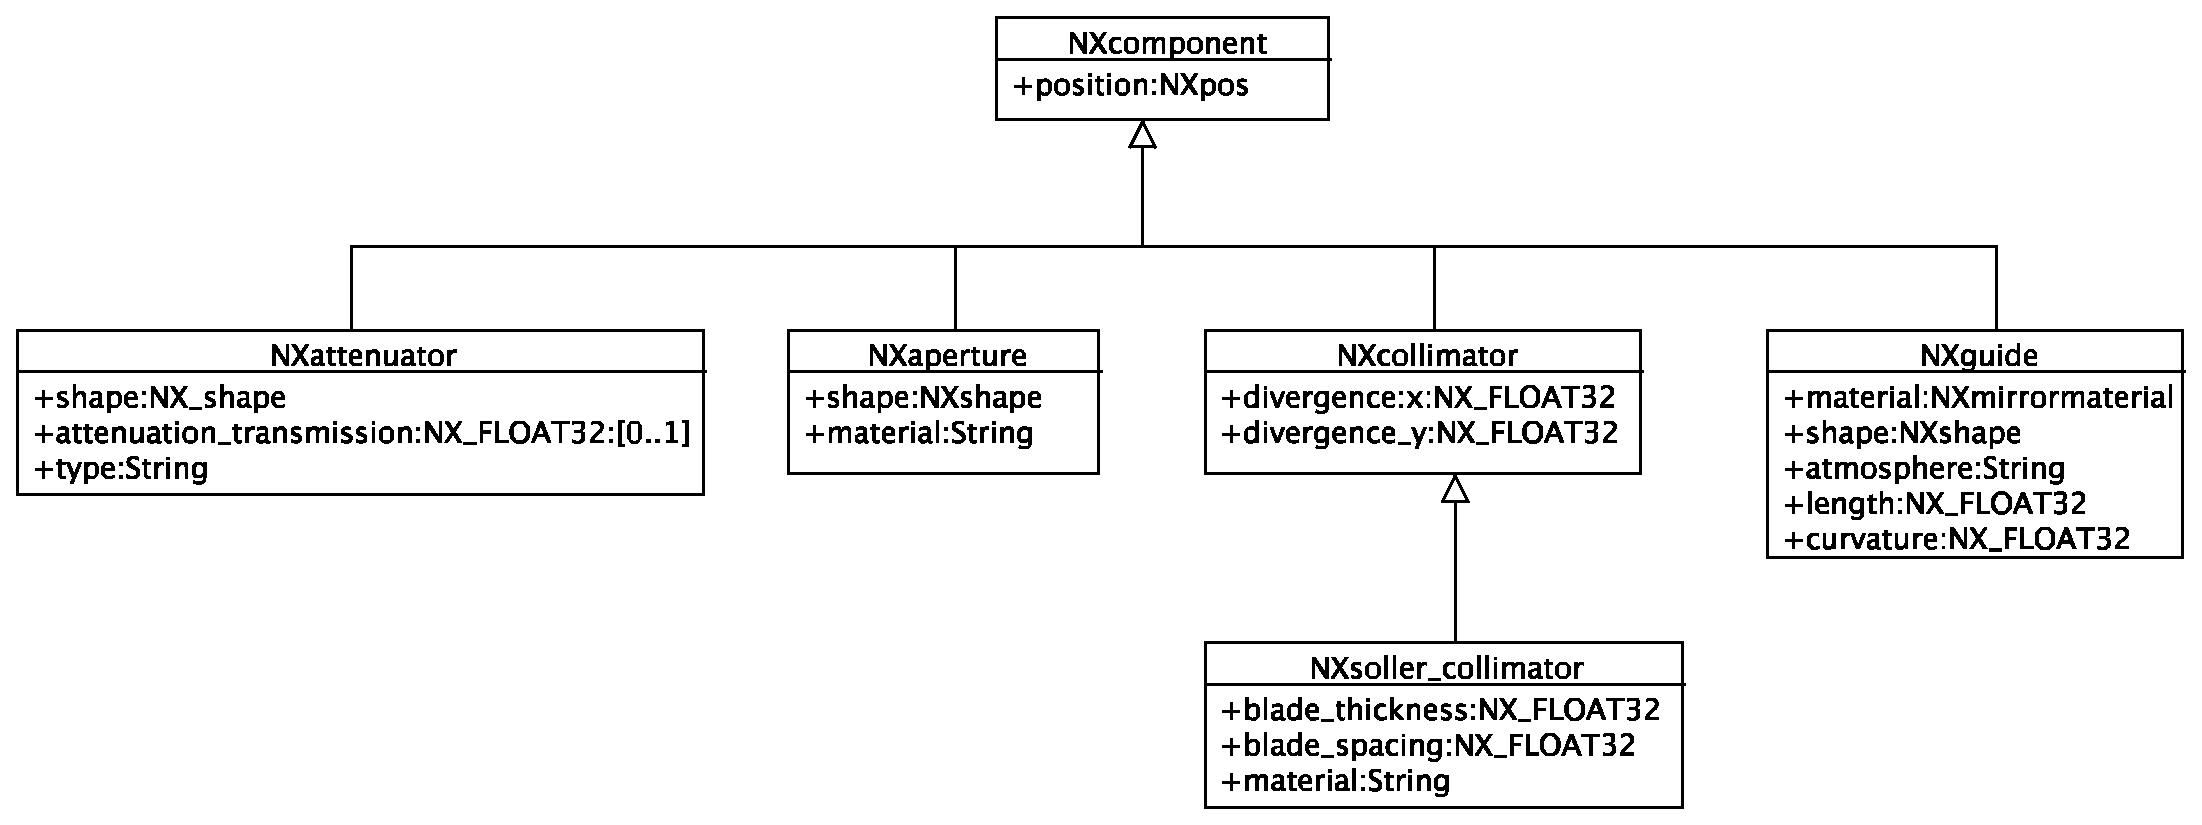
\includegraphics[width=0.75\textwidth]{nxpassivebeam.eps}\end{figure}



\end{center}

\end{slide}\begin{slide}{Active Beam Line Components }
\begin{center}
\begin{figure}
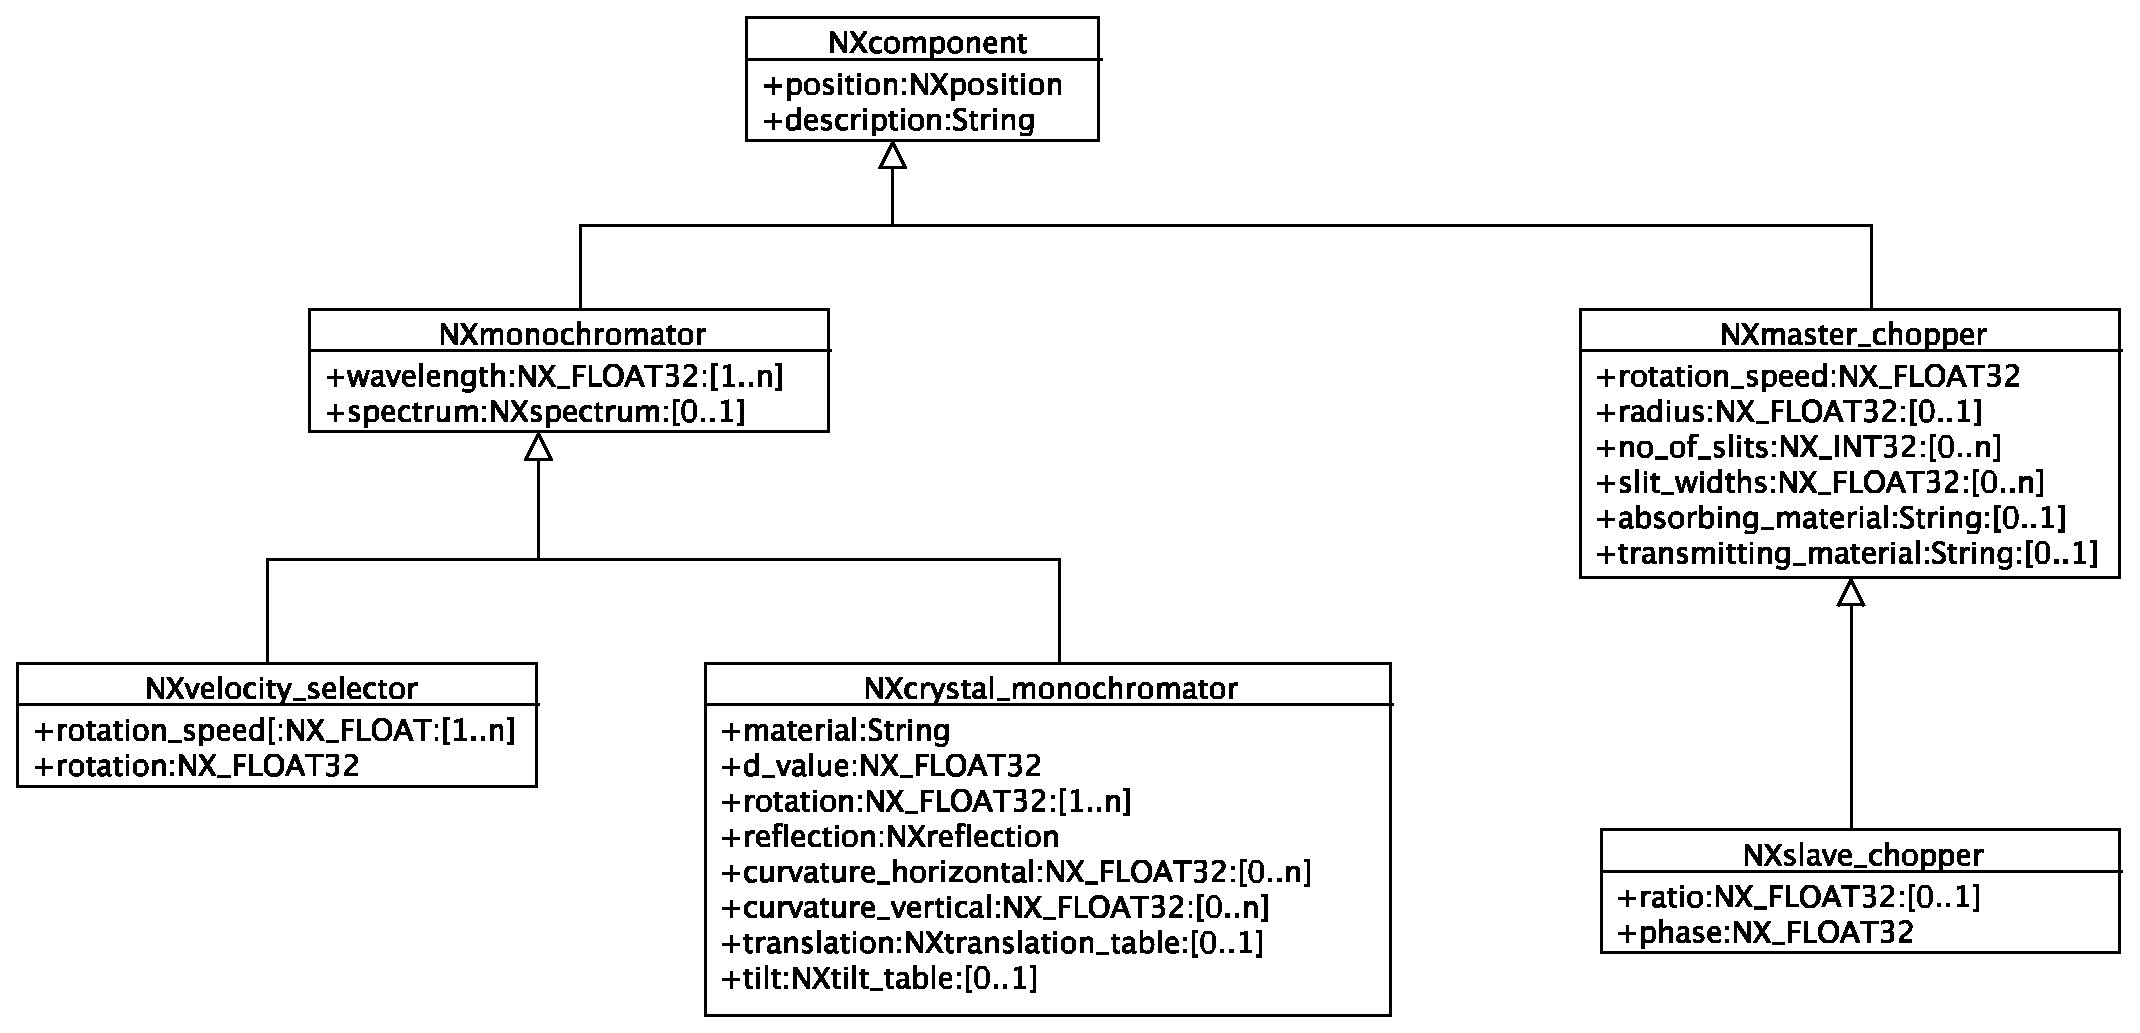
\includegraphics[width=0.75\textwidth]{nxactivebeam.eps}\end{figure}



\end{center}
\end{slide}\begin{slide}{More Beamline Components }
\begin{center}
\begin{figure}
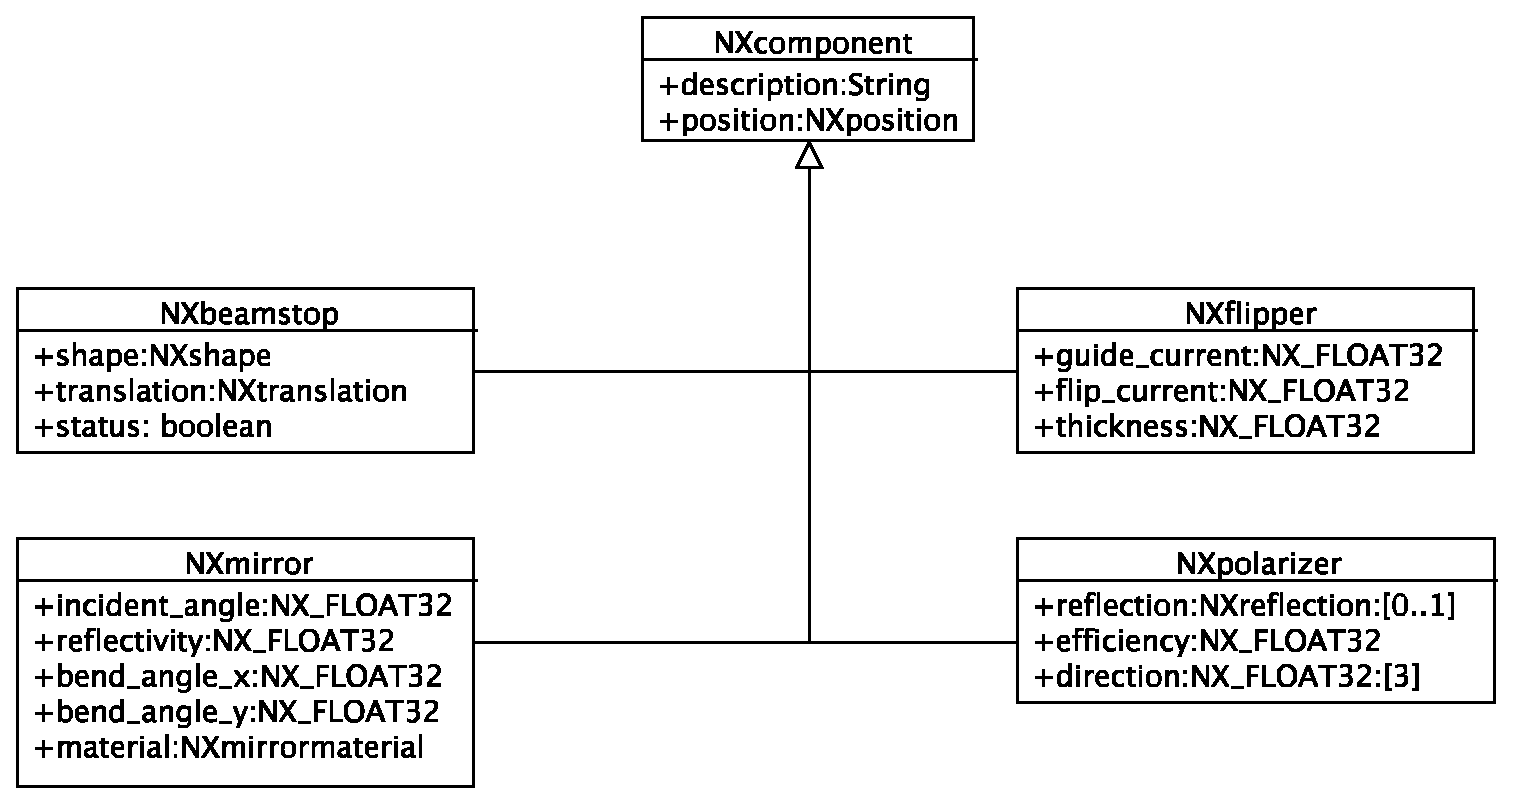
\includegraphics[width=0.75\textwidth]{nxmorebeam.eps}\end{figure}



\end{center}
\end{slide}\begin{slide}{Samples }
\begin{center}
\begin{figure}
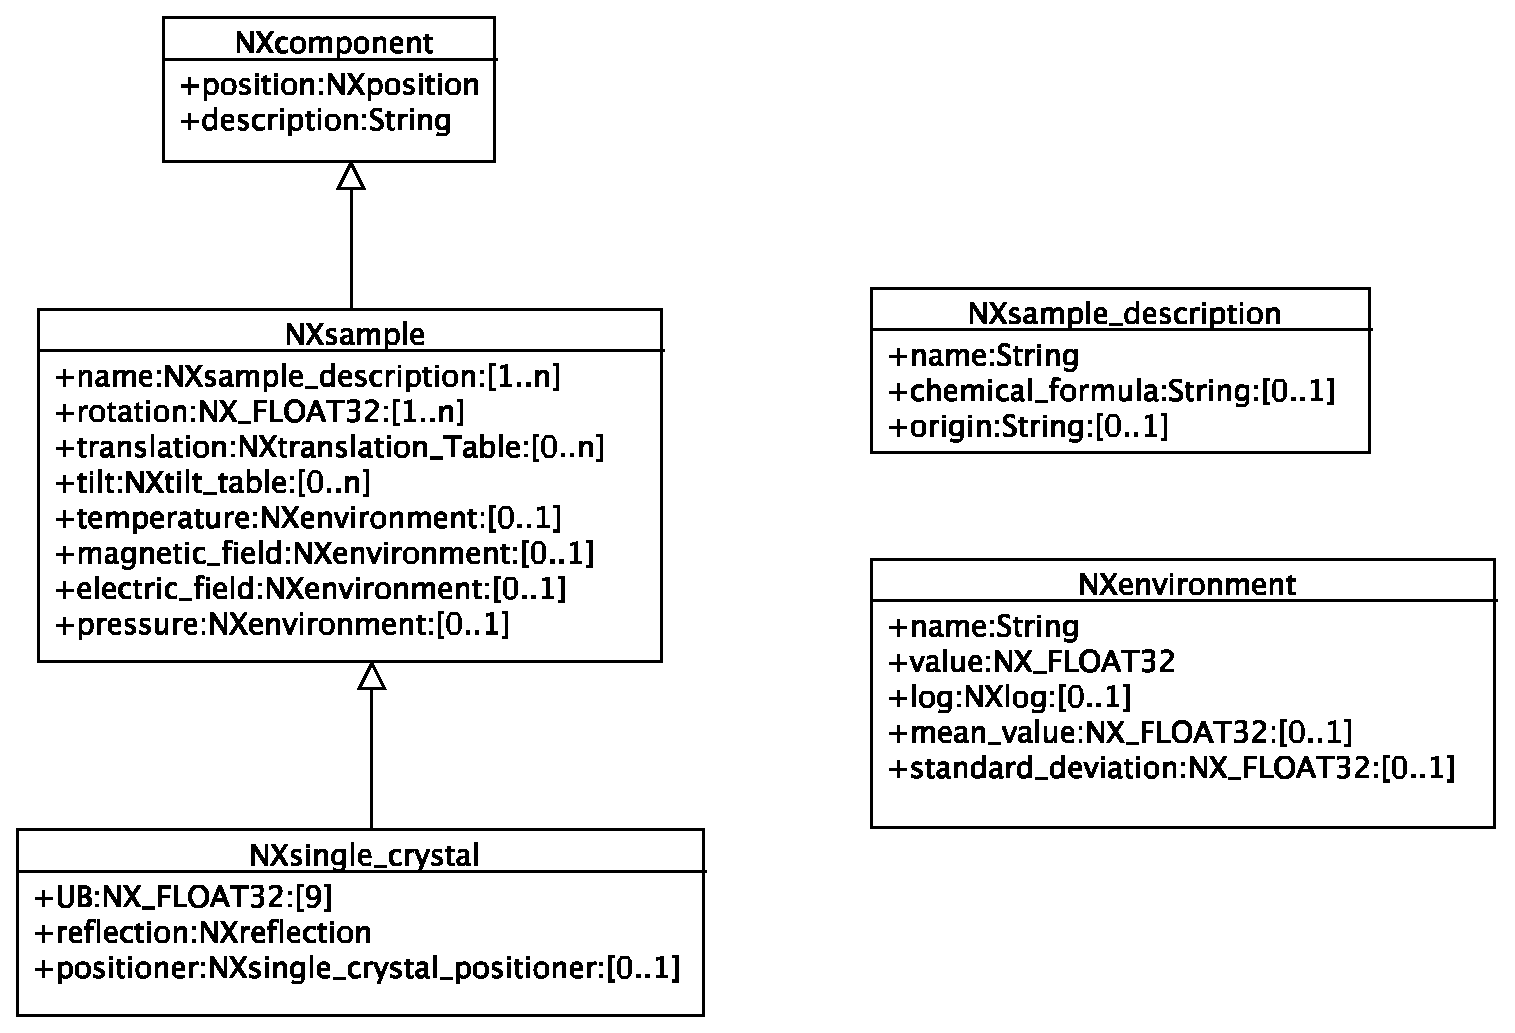
\includegraphics[width=0.75\textwidth]{nxsample.eps}\end{figure}



\end{center}

\end{slide}\begin{slide}{Detectors }
\begin{itemize}\item Concerning data handling there are the following types of detectors:
\begin{itemize}\item single detectors
\item linear detectors
\item area detectors
\item ID detectors 
\end{itemize}\item Detectors have different geometries:
\begin{itemize}\item Detectors can have regular shapes: rectangles, lines etc which are best described as such
\item Some detectors (especially @ ISIS) are highly irregular: Then we need to describe each pixel.
\end{itemize}\item For each detector pixel we need to be able to deduce:
\begin{itemize}\item The scattering angle towards the previous component 
\item The elevation out of the scattering plane
\item The distance to the previous component
\end{itemize}\item All detectors can be described by the general case where we give those values for each pixel
\end{itemize}
\end{slide}\begin{slide}{Non-TOF Detectors }
\begin{center}
\begin{figure}
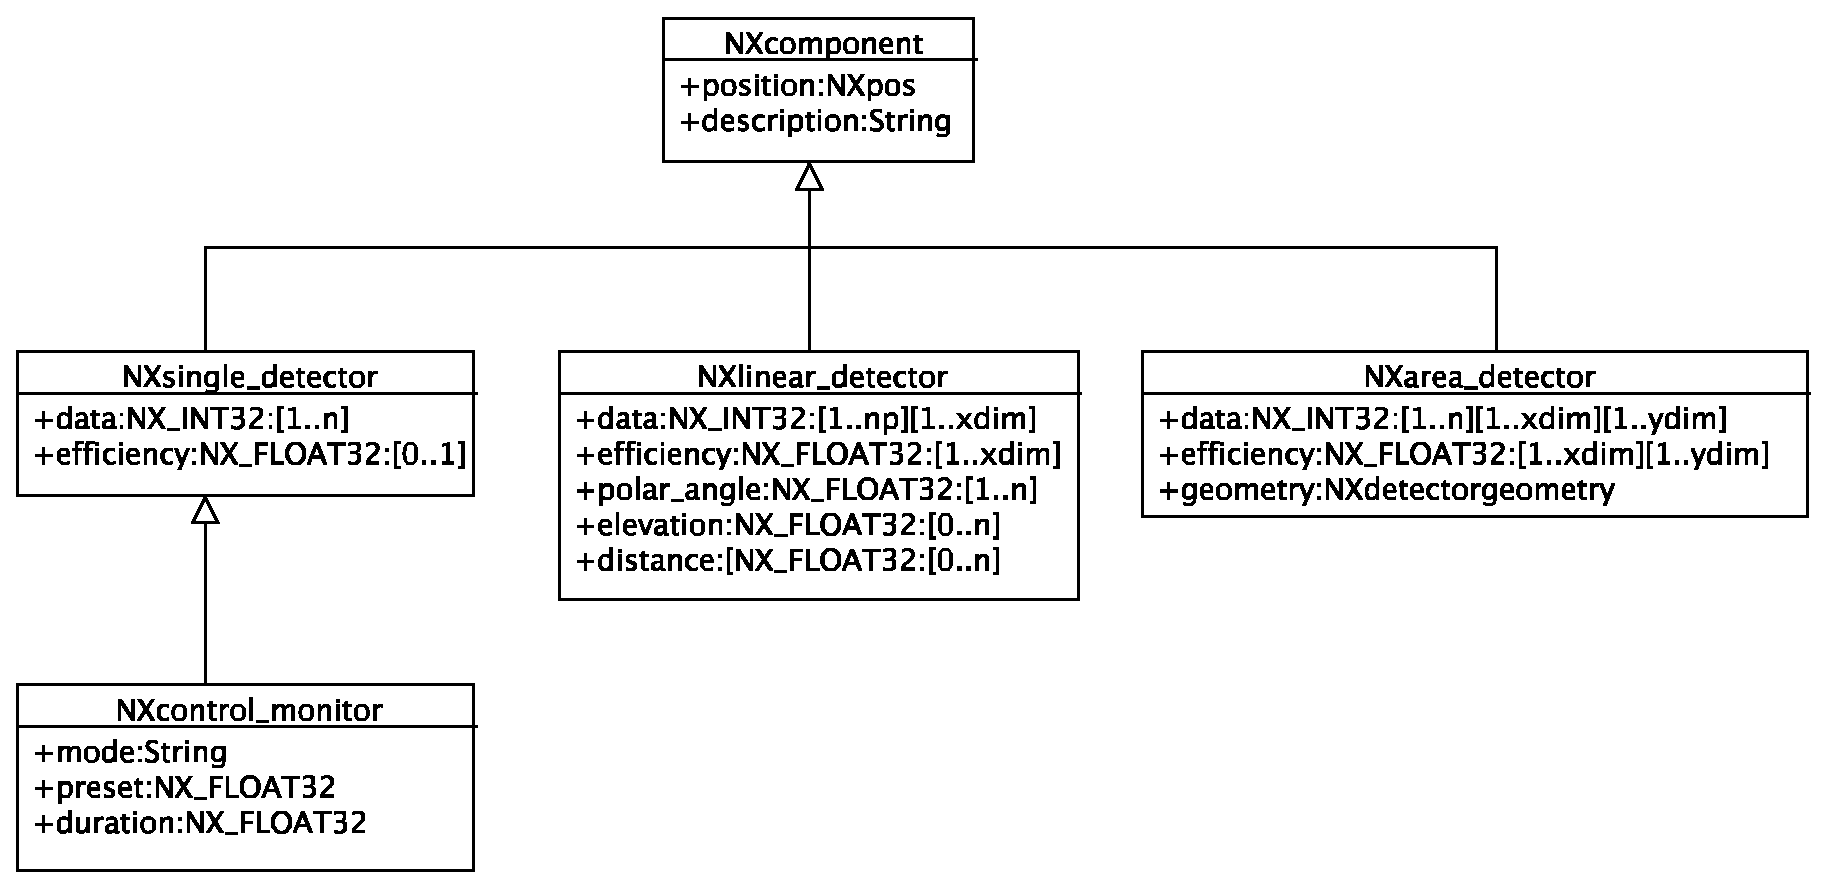
\includegraphics[width=0.75\textwidth]{nxdet.eps}\end{figure}



\end{center}

\end{slide}\begin{slide}{TOF-Detectors }
\begin{center}
\begin{figure}
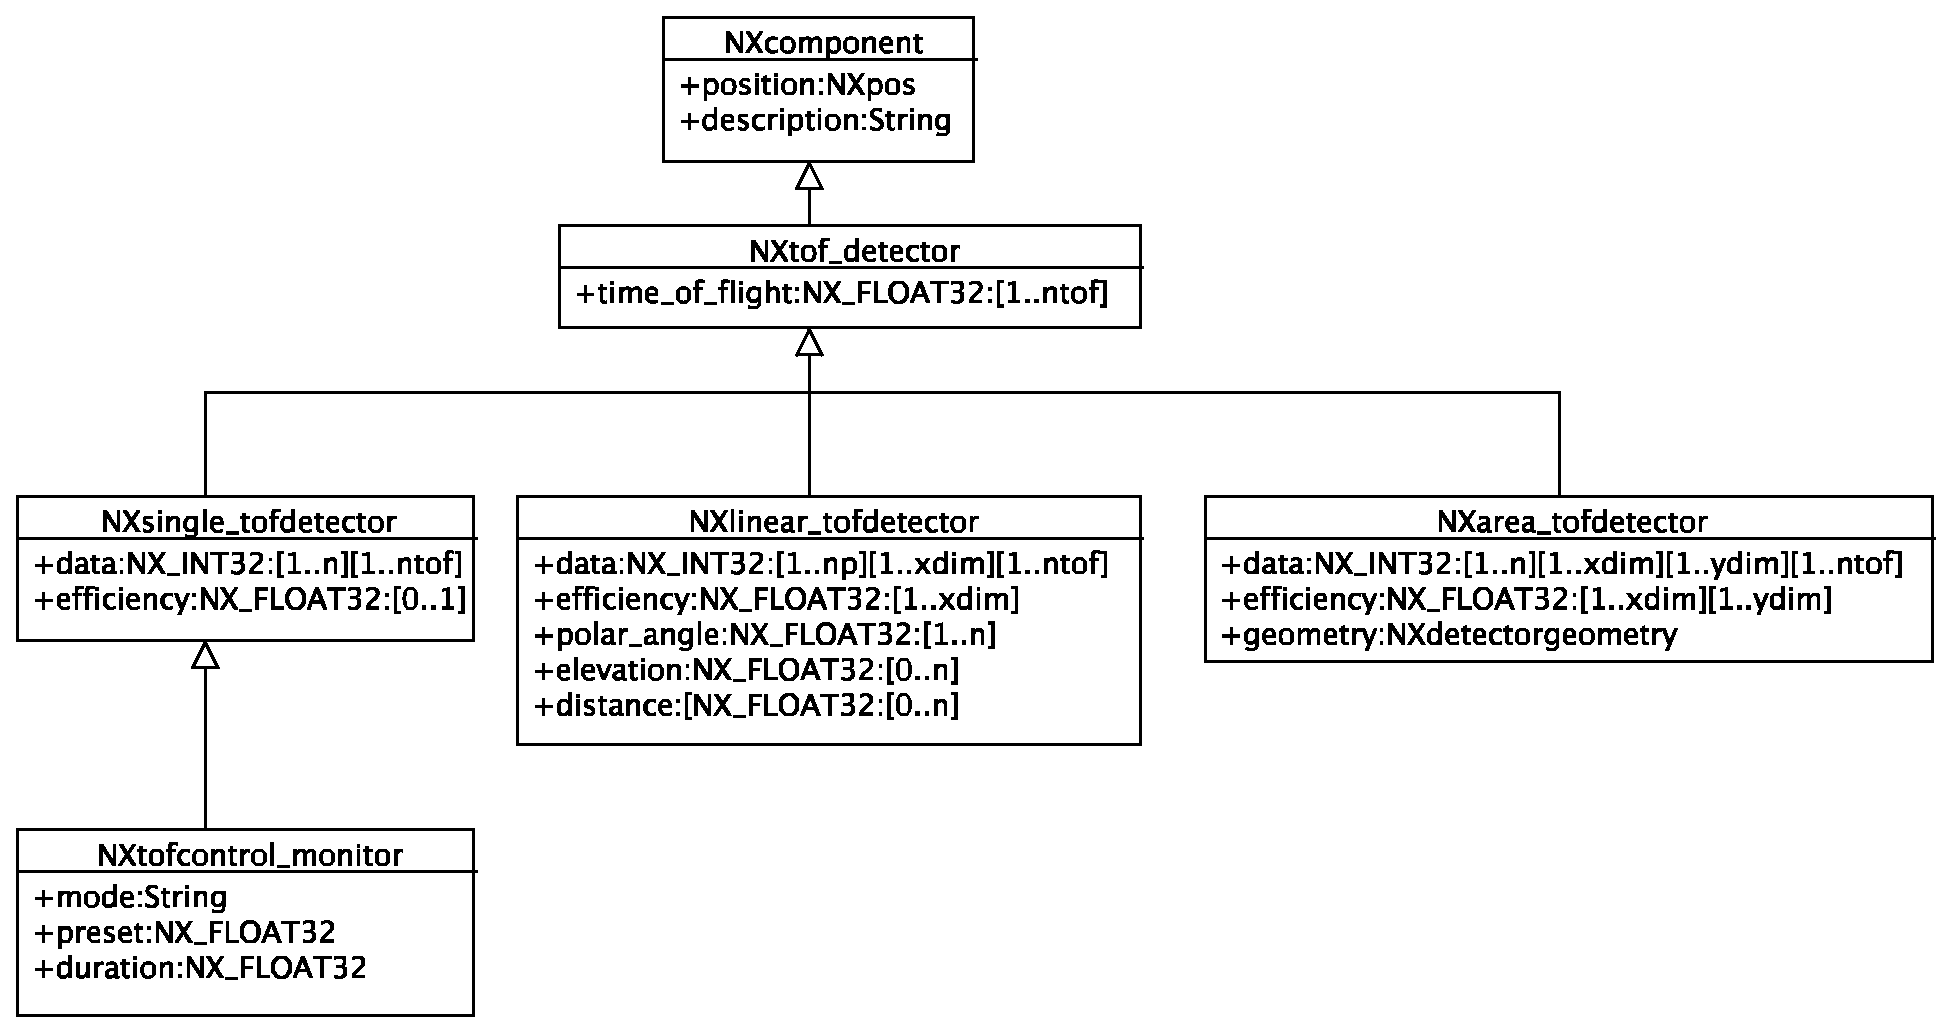
\includegraphics[width=0.75\textwidth]{nxtofdet.eps}\end{figure}



\end{center}

\end{slide}\begin{slide}{More Detectors }
\begin{center}
\begin{figure}
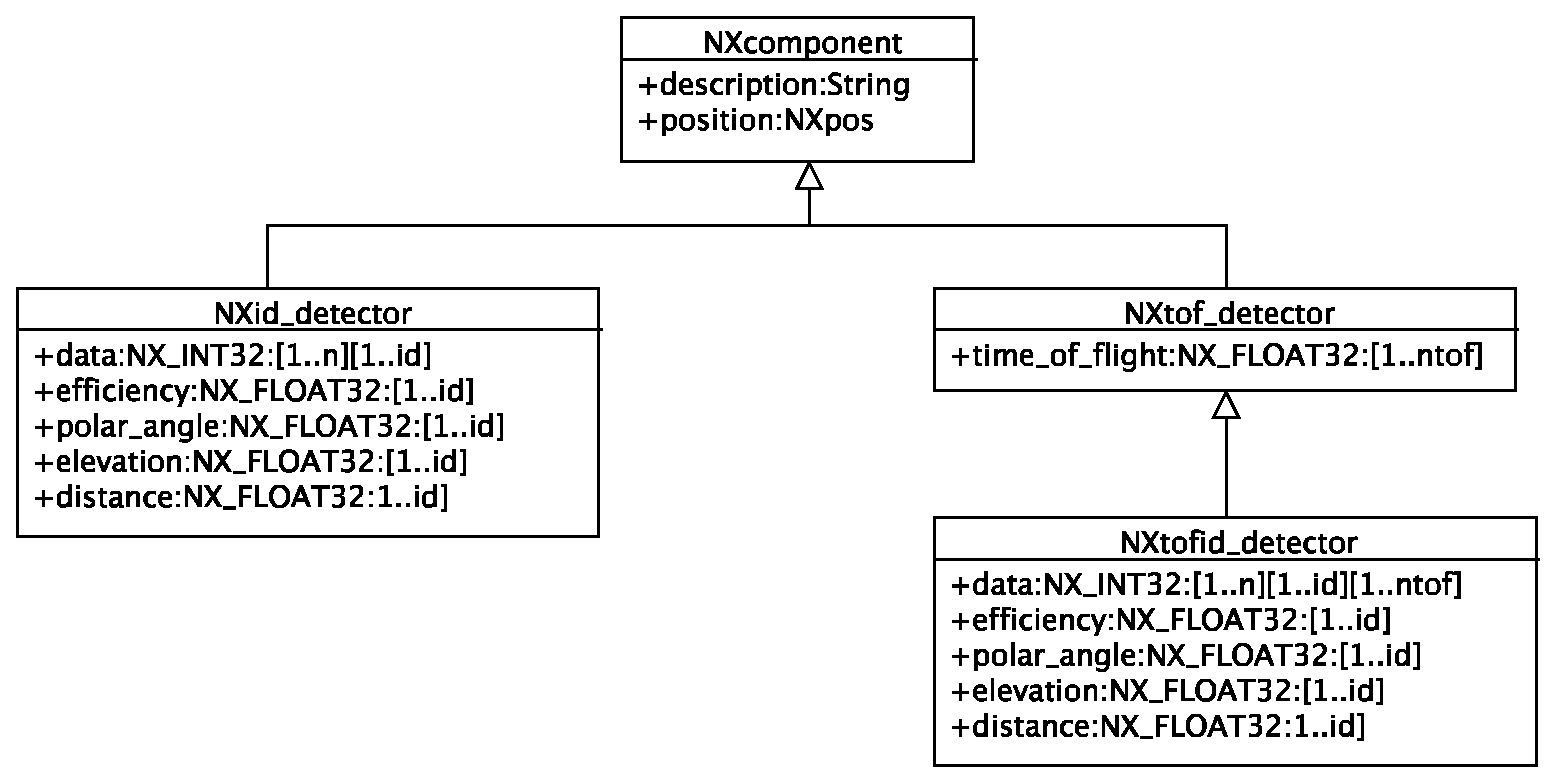
\includegraphics[width=0.75\textwidth]{nxmoredet.eps}\end{figure}



\end{center}

\end{slide}\begin{slide}{Monochromatic Instruments }
\begin{center}
\begin{figure}
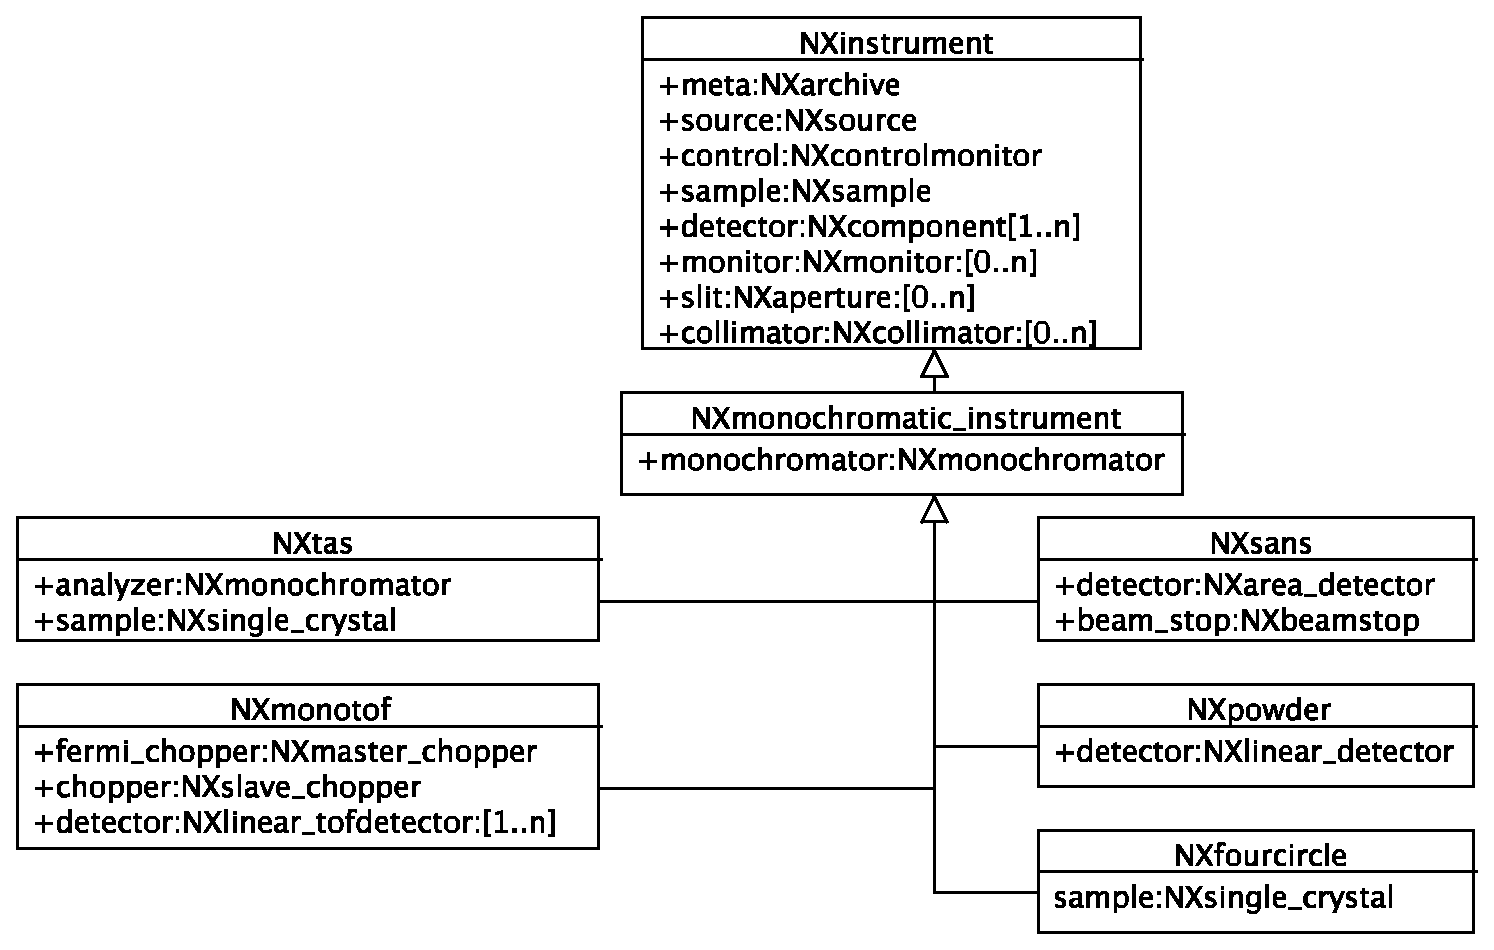
\includegraphics[width=0.75\textwidth]{nxmonoinst.eps}\end{figure}



\end{center}

\end{slide}\begin{slide}{TOF Instruments }
\begin{center}
\begin{figure}
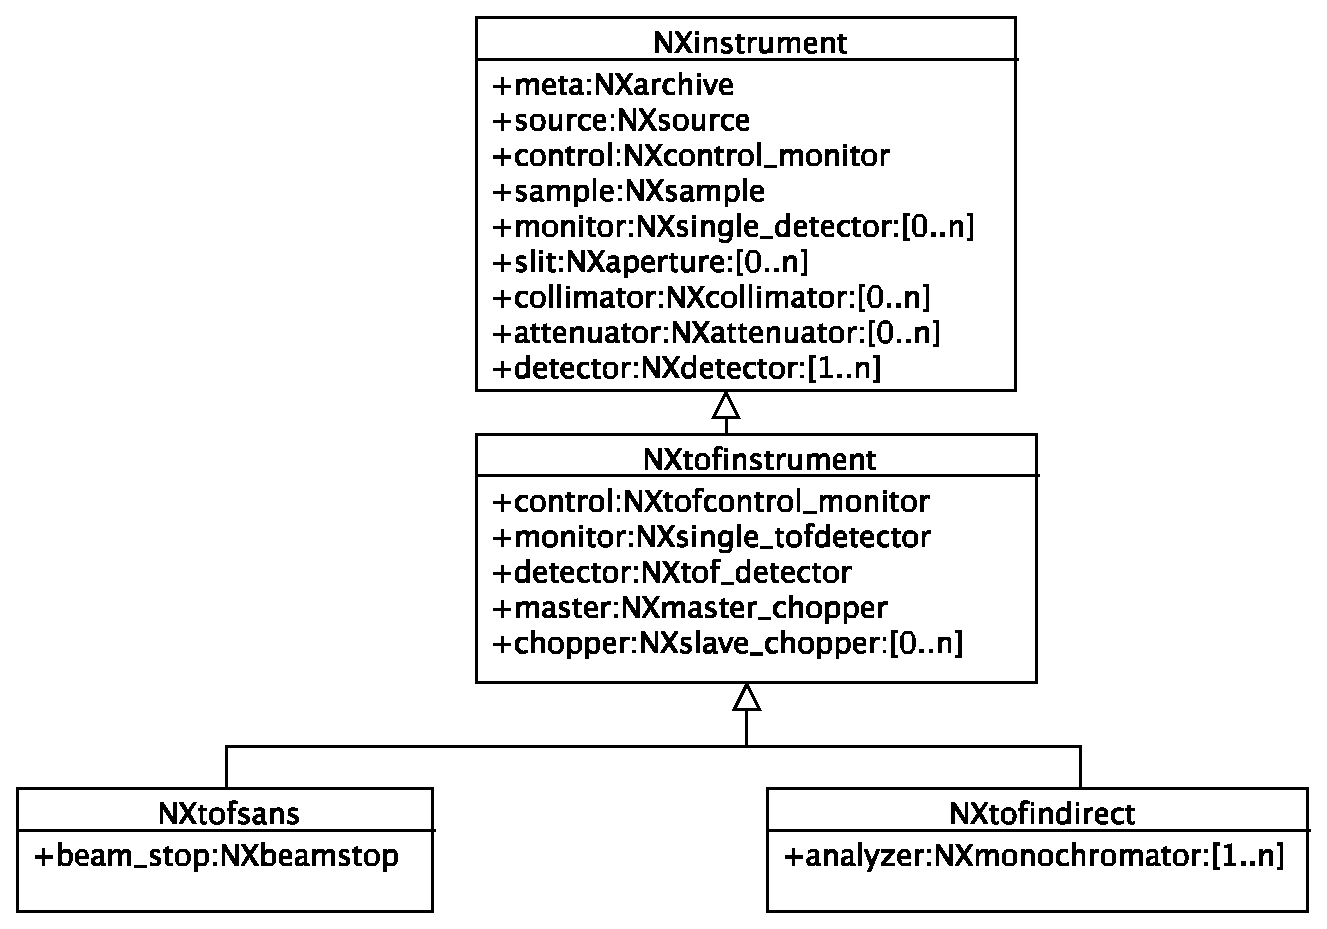
\includegraphics[width=0.75\textwidth]{nxtofinst.eps}\end{figure}



\end{center}

\end{slide}\begin{slide}{Conclusion }
\begin{itemize}\item The current NeXus classes are messy due to lack of specialization
\item More classes improve clarity
\item Inheritance brings better maintainability: for instance adding NXellipitcal as 
 a NXshape does not require changes downstream
\item Caveats:
\begin{itemize}\item backwards compatability diff\mbox{}icult
\item description in XML problematic
\end{itemize}\end{itemize}
















\end{slide}

\end{document}







